\section{Consuntivo di fase}
Il team \textit{clubswendwitch} di seguito espone i dati ottenuti dall'esperienza concreta di sviluppo del progetto.
Vengono evidenziate inoltre le differenze rispetto a quanto esposto nel preventivo analizzato nella sezione precedente. 

\subsection{Analisi}
\newcolumntype{P}[1]{>{\centering\arraybackslash}p{#1}}
{\renewcommand{\arraystretch}{1.8}
    \begin{center}
        \begin{tabular}{P{0.25\linewidth}P{0.15\linewidth}P{0.20\linewidth}}
            \rowcolor[RGB]{33, 73, 50}
            \textcolor{white}{\textbf{Ruolo}} & \textcolor{white}{\textbf{Ore}} & \textcolor{white}{\textbf{Costo}}\\
            \rowcolor[RGB]{216, 235, 171}
            Responsabile & 25 \textcolor{red}{(+5)} & 750\euro \space \textcolor{red}{(+150\euro)}\\
                
            \rowcolor[RGB]{233, 245, 206}
            Amministratore & 20 \textcolor{red}{(+4)}& 400\euro \space \textcolor{red}{(+80\euro)}\\
    
            \rowcolor[RGB]{216, 235, 171}
            Analista & 45 \textcolor{red}{(+5)} & 1125\euro \space \textcolor{red}{(+125\euro)}\\
    
            \rowcolor[RGB]{233, 245, 206}
            Progettista & - & -\\
    
            \rowcolor[RGB]{216, 235, 171}
            Programmatore & - & -\\
    
            \rowcolor[RGB]{233, 245, 206}
            Verificatore & 45 \textcolor{red}{(+5)} & 675\euro \space \textcolor{red}{(+75\euro)}\\
    
            \arrayrulecolor{white}\hline\hline
    
            \rowcolor[RGB]{216, 235, 171}
            Totale Preventivo & 116 & 2520\euro\\
    
            \rowcolor[RGB]{233, 245, 206}
            \textbf{Totale Consuntivo} & 135 \textcolor{red}{(+19)} & 2950\euro \space \textcolor{red}{(+430\euro)}\\
    
        \end{tabular}
    \end{center}
}
\begin{figure}[h!]
	\centering
	\includegraphics[scale=0.70]{../../assets/Diagrammi_Excel/torta_ore_Analisi.png}
	\caption{Ripartizione oraria dei ruoli - Analisi}
\end{figure}

\subsubsection{Considerazioni}
In questa prima fase il gruppo \textit{clubswendwitch} ha visto un incremento delle ore rispetto a quanto riportato nel preventivo. Questo aumento è sicuramente dovuto all'inesperienza generale del gruppo, il quale ha trovato difficoltà nell'analisi del capitolato C5 - Login Warrior e nella conseguente organizzazione dei compiti.\\
\'E però da considerare il fatto che il preventivo redatto è particolarmente ottimista e non tiene conto di eventuali problematiche che poi di fatto si sono presentate.

\subsection{Technology baseline e codifica del PoC}
{\renewcommand{\arraystretch}{2.0}
    \begin{center}
        \begin{tabular}{P{0.25\linewidth}P{0.15\linewidth}P{0.20\linewidth}}
            \rowcolor[RGB]{33, 73, 50}
            \textcolor{white}{\textbf{Ruolo}} & \textcolor{white}{\textbf{Ore}} & \textcolor{white}{\textbf{Costo}}\\
            \rowcolor[RGB]{216, 235, 171}
            Responsabile & 16 \textcolor{red}{(+2)} & 480\euro \space \textcolor{red}{(+60\euro)}\\
                
            \rowcolor[RGB]{233, 245, 206}
            Amministratore & 6 \textcolor{blue}{(-2)} & 120\euro \space \textcolor{blue}{(-40\euro)} \\
    
            \rowcolor[RGB]{216, 235, 171}
            Analista & 12 \textcolor{red}{(+5)} & 300\euro \space \textcolor{red}{(+125\euro)}\\
    
            \rowcolor[RGB]{233, 245, 206}
            Progettista & 25 \textcolor{red}{(+5)} & 625\euro \space \textcolor{red}{(+125\euro)}\\
    
            \rowcolor[RGB]{216, 235, 171}
            Programmatore & 30 \textcolor{red}{(+5)} & 450\euro \space \textcolor{red}{(+75\euro)}\\
    
            \rowcolor[RGB]{233, 245, 206}
            Verificatore & 20 \textcolor{red}{(+5)} & 300\euro \space \textcolor{red}{(+75\euro)}\\
    
            \arrayrulecolor{white}\hline\hline
    
            \rowcolor[RGB]{216, 235, 171}
            Totale Preventivo & 81 & 1735\euro\\
    
            \rowcolor[RGB]{233, 245, 206}
            \textbf{Totale Consuntivo} & 109 \textcolor{red}{(+20)} & 2275\euro \space \textcolor{red}{(+540\euro)}\\
        \end{tabular}
    \end{center}    
}
\begin{figure}[h!]
	\centering
	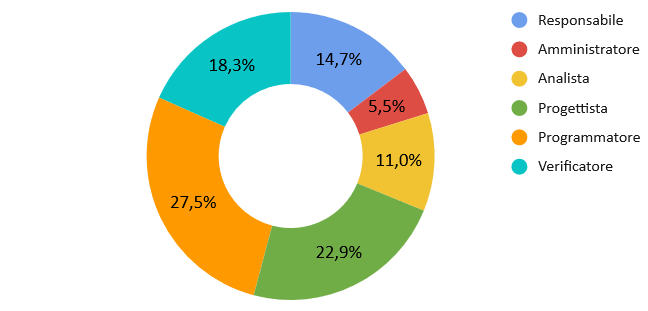
\includegraphics[scale=0.70]{../../assets/Diagrammi_Excel/torta_ore_TB.png}
	\caption{Ripartizione oraria dei ruoli - Technology baseline}
\end{figure}

\subsection{Considerazioni}
In questa fase il gruppo \textit{clubswendwitch} ha riscontrato un incremento delle ore su quasi tutti i ruoli ad eccezione del ruolo di amministratore. Le motivazioni che hanno portato all'aumentare delle ore necessarie sono sicuramente: l'inesperienza del gruppo con le tecnologie utilizzate (come \textit{React}$^{G}$ e \textit{D3.js}$^{G}$), l'attuale situazione pandemica infatti un membro del gruppo sfortunatamente è risultato positivo al covid e l'accavallarsi degli esami universitari.\\
L'unico ruolo che ha migliorato le aspettative è stato l'amministratore, infatti gli strumenti di organizzazione delle tasks funzionano egregiamente e questo ha semplificato molto il lavoro, portando ad una riduzione sul consuntivo di fase di circa due ore.

\subsection{Riepilogo consuntivo}
{\renewcommand{\arraystretch}{2.0}
        \begin{tabular}{P{0.25\linewidth}P{0.07\linewidth}P{0.07\linewidth}P{0.07\linewidth}P{0.08\linewidth}P{0.08\linewidth}P{0.08\linewidth}P{0.08\linewidth}}
            \rowcolor[RGB]{33, 73, 50}
            \textcolor{white}{\textbf{Nominativo}} & \textcolor{white}{\textbf{RE}} &
            \textcolor{white}{\textbf{AM}} & \textcolor{white}{\textbf{AN}} &
            \textcolor{white}{\textbf{PT}} & \textcolor{white}{\textbf{PG}} &
            \textcolor{white}{\textbf{VE}} & \textcolor{white}{\textbf{Tot.}}\\
        
            \rowcolor[RGB]{216, 235, 171}
            Barilla Gianmarco & 0 \par \textcolor{blue}{(-2)} &  & & & & & \\
            
            \rowcolor[RGB]{233, 245, 206}
            Beni Valentina & 13 \par \textcolor{red}{(+4)} &  & & & & & \\

            \rowcolor[RGB]{216, 235, 171}
            Bustaffa Marco & 15 \par \textcolor{red}{(+5)}&  & & & & & \\

            \rowcolor[RGB]{233, 245, 206}
            Canel Alessandro & 0 &  & & & & & \\

            \rowcolor[RGB]{216, 235, 171}
            Ferrarini Alessio & 4 &  & & & & & \\

            \rowcolor[RGB]{233, 245, 206}
            Pozzebon Samuele & 9 &  & & & & & \\

            \arrayrulecolor{white}\hline\hline

            \rowcolor[RGB]{216, 235, 171}
            Totale ore ruolo & 41 &  & & & & & \\

            \rowcolor[RGB]{233, 245, 206}
            Totale costi ruolo &  &  & & & & & \\




        \end{tabular}
}






% TO DO: METTERE LE CAPTIONS ALLE TABELLE
